\begin{figure*}[t]
\small
\setlength{\tabcolsep}{3pt}
\centering
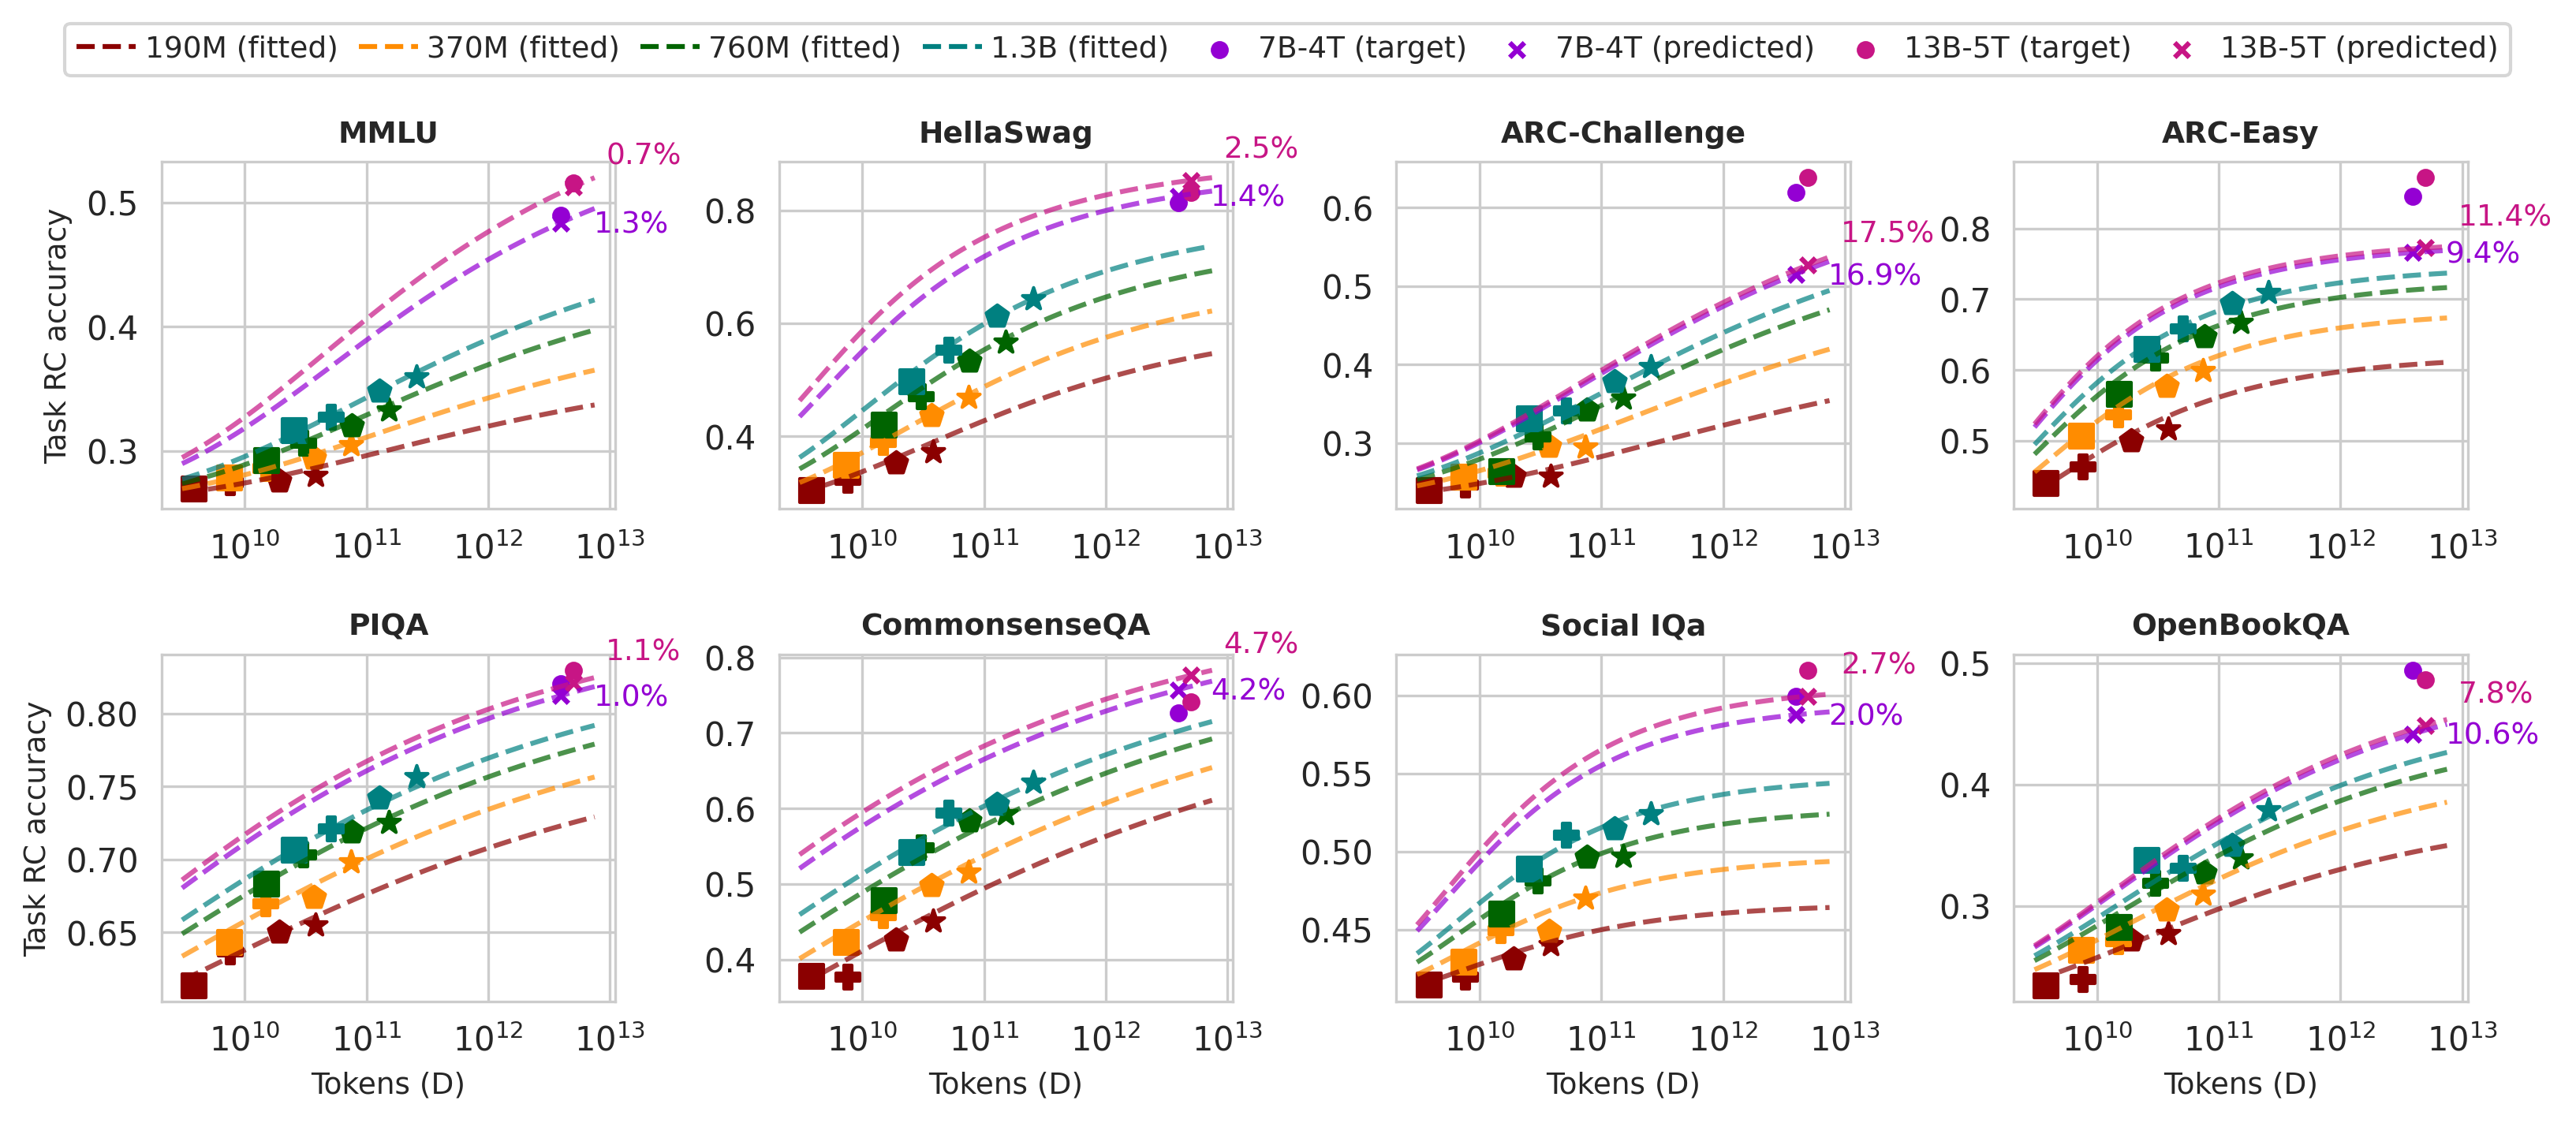
\includegraphics[scale=0.5]{images/chained_main.png}
\resizebox{0.75 \textwidth}{!}{%
\begin{tabular}{l c r | r r r r | r r r r}
\toprule
& & & \multicolumn{4}{c}{\textbf{7B-4T}} & \multicolumn{4}{c}{\textbf{13B-5T}}\\
\textbf{Task} & \textbf{Split} & \textbf{Examples} & Pred & Actual & Error & \%Error & Pred & Actual & Error & \%Error \\
\midrule
MMLU & test & 14,042 & 48.4 & 49.0 & 0.6 & 1.3\% & 51.3 & 51.6 & 0.3 & 0.7\% \\
HellaSwag & val & 10,042 & 82.5 & 81.3 & 1.2 & 1.4\% & 85.3 & 83.2 & 2.1 & 2.5\% \\
ARC-Challenge & test & 1,172 & 51.5 & 61.9 & 10.4 & 16.9\% & 52.7 & 63.8 & 11.1 & 17.5\% \\
ARC-Easy & test & 2,376 & 76.6 & 84.6 & 8.0 & 9.4\% & 77.2 & 87.2 & 10.0 & 11.4\% \\
PIQA & val & 1,838 & 81.2 & 82.0 & 0.8 & 1.0\% & 82.1 & 83.0 & 0.9 & 1.1\% \\
CommonsenseQA & val & 1,221 & 75.7 & 72.6 & 3.1 & 4.2\% & 77.6 & 74.1 & 3.5 & 4.7\% \\
Social IQa & val & 1,954 & 58.7 & 59.9 & 1.2 & 2.0\% & 59.9 & 61.6 & 1.7 & 2.7\% \\
OpenBookQA & test & 500 & 44.2 & 49.4 & 5.2 & 10.6\% & 44.9 & 48.6 & 3.7 & 7.8\% \\
\midrule
Average & -- & -- & -- & -- & 3.8 & 5.9\% & -- & -- & 4.2 & 6.1\% \\
\bottomrule
\end{tabular}
}%
\caption{
Task accuracy prediction for the target models using task loss as the intermediate feature.
\ding{110} = 1xC; \ding{58} = 2xC; $\pentagofill$ = 5xC; $\bigstar$ = 10xC.
Prediction error is next to the target.
}
\label{tab:stacked_pred}
\vspace{-8pt}
\end{figure*}
